\documentclass[11pt]{article}
 
\usepackage[margin=1in]{geometry}
\usepackage{amsmath,amsthm,amssymb}
\usepackage{graphics}
\usepackage{graphicx}
\usepackage{subcaption}
\usepackage[colorlinks]{hyperref}
\usepackage{changepage}
 
\newcommand{\N}{\mathbb{N}}
\newcommand{\R}{\mathbb{R}}
\newcommand{\Z}{\mathbb{Z}}
\newcommand{\Q}{\mathbb{Q}}
 
\newenvironment{theorem}[2][Theorem]{\begin{trivlist}
\item[\hskip \labelsep {\bfseries #1}\hskip \labelsep {\bfseries #2.}]}{\end{trivlist}}
\newenvironment{lemma}[2][Lemma]{\begin{trivlist}
\item[\hskip \labelsep {\bfseries #1}\hskip \labelsep {\bfseries #2.}]}{\end{trivlist}}
\newenvironment{exercise}[2][Exercise]{\begin{trivlist}
\item[\hskip \labelsep {\bfseries #1}\hskip \labelsep {\bfseries #2.}]}{\end{trivlist}}
\newenvironment{problem}[2][Problem]{\begin{trivlist}
\item[\hskip \labelsep {\bfseries #1}\hskip \labelsep {\bfseries #2.}]}{\end{trivlist}}
\newenvironment{question}[2][Question]{\begin{trivlist}
\item[\hskip \labelsep {\bfseries #1}\hskip \labelsep {\bfseries #2.}]}{\end{trivlist}}
\newenvironment{corollary}[2][Corollary]{\begin{trivlist}
\item[\hskip \labelsep {\bfseries #1}\hskip \labelsep {\bfseries #2.}]}{\end{trivlist}}
 
\begin{document}
 
\title{CS281A - Problem Set 2}
\author{Andrea Bajcsy}
 
\maketitle
 
\begin{problem}{2.1}
\text{ }\\

(a) We can formulate the polynomial regression problem as a form of linear prediction by soliving the general linear model equation $X\alpha = y$ where:
\\
\[
X=
  \begin{bmatrix}
    1 & t_{1} & t^2_{1} & ... & t^D_{1}\\
    1 & t_{2} & t^2_{2} & ... & t^D_{2}\\
    1 & t_{3} & t^2_{3} & ... & t^D_{3}\\
    ...\\
    1 & t_{n} & t^2_{n} & ... & t^D_{n}\\
  \end{bmatrix}
\alpha=
	\begin{bmatrix}
		\alpha_{1}\\
		\alpha_{2}\\
		\alpha_{3}\\
		...\\
		\alpha_{D}\\
	 \end{bmatrix}
y=
	\begin{bmatrix}
		y_{1}\\
		y_{2}\\
		y_{3}\\
		...\\
		y_{n}\\
	 \end{bmatrix}
\]

(b) Figure \ref{fig:2b} shows a plot of the mean-squared error R(D) vs. Degree $D \in {1,2,...n-1}$ when using the data in y.dat and t.dat. See back for code that performs least-squares fit of a polynomial of degree D. 
\begin{figure}[h!]
  \centering
  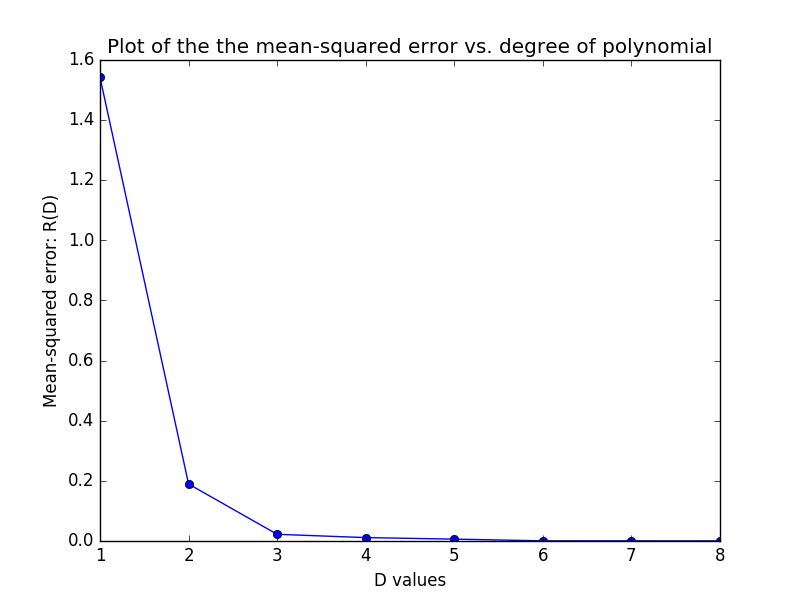
\includegraphics[scale=0.5]{figs/2b.png}
  \caption{D vs. R(D)}
  \label{fig:2b}
\end{figure}

(c) 
{\color{red} How does the MSE behave as a function of D and why?}
With the degree n-1 fit, we get (approximately) zero mean-squared error since the function fits exactly to every data point. 
{\color{red}What happens if you try to fit a polynomial of degree n? Why? To fit a polynomial of degree n, we will be solving $X\alpha = y$, where $X^{n~x~n}$.
\[
	\begin{bmatrix}
	1 & t_{1} & t^2_{1} & ... & t^n_{1}\\
	1 & t_{2} & t^2_{2} & ... & t^n_{2}\\
	1 & t_{3} & t^2_{3} & ... & t^n_{3}\\
	...\\
	1 & t_{n} & t^2_{n} & ... & t^n_{n}\\
	\end{bmatrix}
	\begin{bmatrix}
		\alpha_{1}\\
		\alpha_{2}\\
		\alpha_{3}\\
		...\\
		\alpha_{n}\\
	 \end{bmatrix}
=
	\begin{bmatrix}
		y_{1}\\
		y_{2}\\
		y_{3}\\
		...\\
		y_{n}\\
	 \end{bmatrix}
\]
Using ordinary least-squares, we solve for $\alpha$ = $(X^{T}X)^{-1}X^{T}y$.}

(d) Figure \ref{fig:2d} shows a plot of the degree $D \in {1,2,...n-1}$ versus the mean-squared error R(D) and $\tilde{R}$ when using the data in y.dat, yfresh.dat, and t.dat.  {\color{red}Why do you think that this plot is qualitatively different from the plot in part (b)?} Even though we are fitting D = n-1 degree polynomial to the new yfresh.dat data, the model was trained on y.dat and will approximate yfresh.dat with greater error than the data it was trained on and cannot be a perfect estimator. Thus, the error appears to plateu for the same values of D with yfresh.dat or y.dat but at a higher error value when using yfresh.dat. {\color{red}What does this tell you how the fitted degree D should be chosen?} Choose the minimal degree D after which the error doesn't change within some small $\epsilon$ bound. 
\begin{figure}[h!]
  \centering
  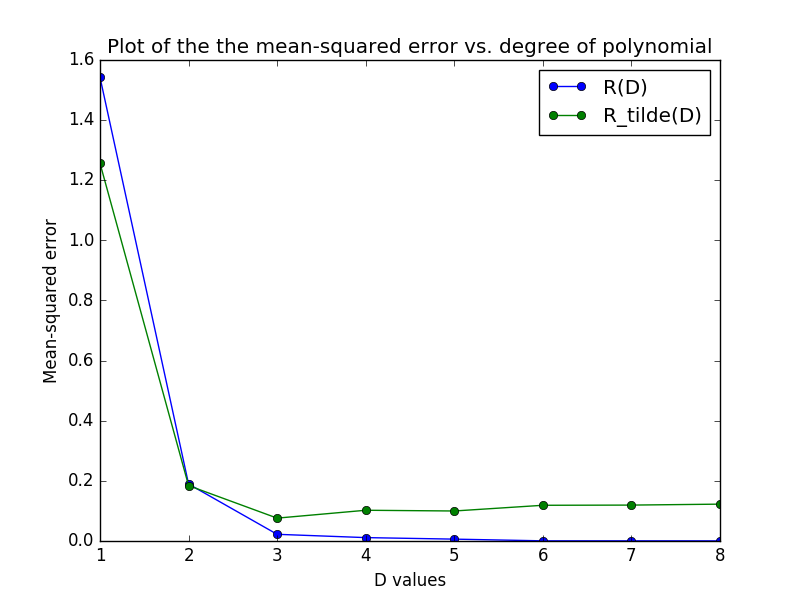
\includegraphics[scale=0.5]{figs/2d.png}
  \caption{D vs. R(D) and $\tilde{R}$}
  \label{fig:2d}
\end{figure}

(e) Figure \ref{fig:2e} shows a plot of the degree $D \in {2,...9}$ versus the mean-squared error $\tilde{R}$ and F(D) when using the data in y.dat, yfresh.dat, and t.dat. {\color{red}How are the minimizing arguments of the two functions related?} {\color{red}Why is this an interesting observation?}
\begin{figure}[h!]
  \centering
  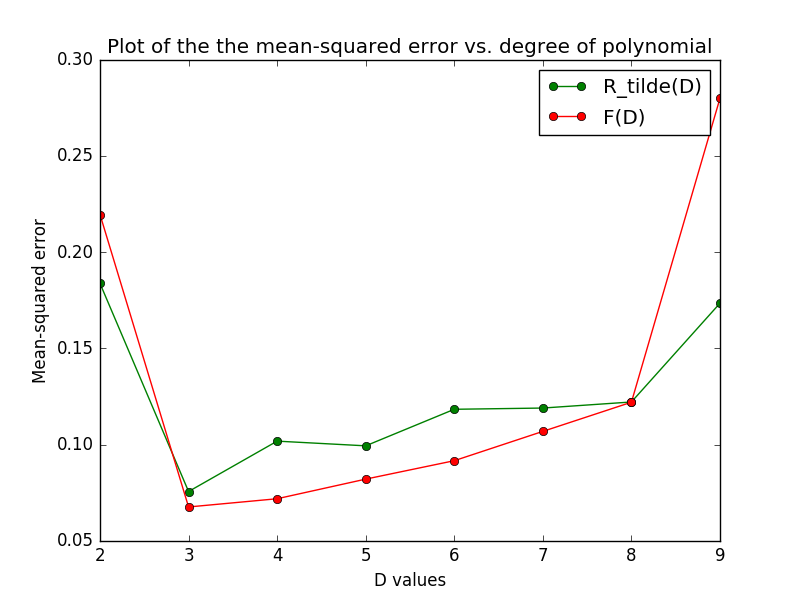
\includegraphics[scale=0.5]{figs/2e.png}
  \caption{D vs. $\tilde{R}$ and F(D)}
  \label{fig:2e}
\end{figure}

\end{problem}
 
\begin{problem}{2.2}
\text{ }\\

(a) Prove that A is a convex function.
\begin{proof}
By definition, 
\[ A(\eta) = log(\int_\gamma h(y)e^{\eta y}\,dy )~~,~~p_{\eta}(y) = h(y)e^{\eta y-A(\eta)} \]
To prove convexity, we want to take the second derivative. Let:
\[B(\eta) = \int_\gamma h(y)e^{\eta y}\,dy \]
Then the first derivative we get:
\[ \frac{\partial A(\eta)}{\partial \eta}
   = \left( \frac{1}{B(\eta)}\right)
     \left(\frac{\partial B(\eta)}{\partial \eta}\right) 
   = \frac{\int_\gamma h(y)e^{\eta y} y \,dy}{\int_\gamma h(y)e^{\eta y}\,dy}
   = \frac{\int_\gamma h(y)e^{\eta y - A(\eta)} y \,dy}{\int_\gamma h(y)e^{\eta y - A(\eta)}\,dy}
   =E_{p_{\eta}}[y]\]
Taking the second derivative we have:
\[ \frac{\partial}{\partial \eta}~\frac{B'(\eta)}{B(\eta)}
   = \frac{\partial}{\partial \eta}\left( B'(\eta)\frac{1}{B(\eta)}\right)
   = \frac{B''(\eta)}{B(\eta)} - \frac{(B'(\eta))^2}{B(\eta)^2}\]
\[= \frac{\int_\gamma h(y)e^{\eta y} y^2 \,dy}{\int_\gamma h(y)e^{\eta y}\,dy}~-~(E_{p_{\eta}}[y])^2
   = \frac{\int_\gamma h(y)e^{\eta y - A(\eta)} y \,dy}{\int_\gamma h(y)e^{\eta y - A(\eta)}\,dy}~-~(E_{p_{\eta}}[y])^2\]
\[ = E_{p_{\eta}}[y^2]~-~(E_{p_{\eta}}[y])^2 
   = Var_{p_{\eta}}[y] ~\succeq~0 \]

Since $Var_{p_{\eta}}$ is positive definite, we have shown that $A(\eta)$ is convex.
\end{proof}

(b) Express KL divergance in terms of $A(\eta)$ and $A'(\eta)$. 

\[ D(p_{\eta} || p_{\eta}) = E_{\eta} \left(log(\frac{h(y)e^{\eta y - A(\eta)}}{h(y)e^{\tilde \eta y - A(\tilde \eta)}})\right)\]
\[= \int_y log \left(e^{(\eta - \tilde{n})y - (A(\eta) - A(\tilde{\eta}))} p_{\eta}(y) \right) \,dy \]
\[= \int_y \left((\eta - \tilde{n})y - (A(\eta) - A(\tilde{\eta})\right) h(y)e^{\eta y - A(\eta)} \,dy \]
\[= (\eta - \tilde{n})\int_y h(y)e^{\eta y - A(\eta)}y \,dy - (A(\eta) - A(\tilde{\eta})) \int_y h(y)e^{\eta y - A(\eta)} \,dy \]
\[= (\eta - \tilde{n})A' - A(\eta) + A(\tilde{\eta}) \]

Since $A\ = \int_y h(y)e^{\eta y - A(\eta)}y $ and $\int_y p_{\eta}(y)dy = 1 $ by definition.
\\

(i) Bernoulli random variable:
\\
\[p_{\eta}(y) = \eta^{y}(1-\eta)^{1-y}, y \in {0,1}, n \in (0,1)\]
\[ = e^{ylog(\eta) + (1-y)log(1-\eta)} = e^{ylog(\frac{\eta}{1-\eta}) - log(1+e^{\frac{\eta}{1-\eta}})}\]

\begin{adjustwidth}{2.5em}{0pt}
Thus, we have $A(\eta) = log(1+e^{\eta})$ and $A^{*}(t) = sup_{\eta\in R}~ \left\{\eta t - log(1+e^{\eta}\right\}$. We now take the gradient of $A^{*}$ with respect to $\eta$, set this to 0 in order to solve the optimization problem, and then solve for $\eta$ in terms of $t$.
\end{adjustwidth}

\[\nabla_{\eta} A^{*}(t) = t - \frac{e^{\eta}}{1+e^{\eta}} \]
\[0  = t - \frac{e^{\eta}}{1+e^{\eta}} \implies t = \frac{e^{\eta}}{1+e^{\eta}} \]
\[ \frac{1}{t} = \frac{1+e^{\eta}}{e^{\eta}} = \frac{1}{e^{\eta}} + 1 \implies \frac{1}{t} - 1 = \frac{1}{e^{\eta}}\]
\[e^{\eta} = \frac{1}{\frac{1}{t} - 1} \implies \eta = log(\frac{1}{\frac{1}{t} - 1})\]
\[\eta = -log(\frac{1}{t} - 1))\]

\begin{adjustwidth}{2.5em}{0pt}
Substituting this back into our equation, we get:
\end{adjustwidth}

\[A^{*}(t) = -tlog(\frac{1}{t}-1) - log(1+e^{-log(\frac{1}{t}-1)}) = -tlog(\frac{1}{t}-1) + log(1-t)\]
\[= tlog(t) - tlog(1-t) + log(1-t) = tlog(t) + (1-t)log(1-t)\]

(ii) Gaussian random variable:
\\
\[p_{\eta}(y) = \frac{e^{\frac{-y^{2}}{2}}}{\sqrt{2\pi}}e^{yn - \frac{\eta^2}{2}}\]

\begin{adjustwidth}{2.5em}{0pt}
Thus, we have $A(\eta) = \frac{\eta^2}{2}$ and $A^{*}(t) = sup_{\eta\in R}~ \left\{\eta t - \frac{\eta^2}{2}\right\}$. 
\end{adjustwidth}

\[\nabla_{\eta} A^{*}(t) = t - n \]
\[0 = t - n \implies t = n \]

\begin{adjustwidth}{2.5em}{0pt}
Substituting this back into our equation, we get:
\end{adjustwidth}
\[A^{*}(t) = t^2 - \frac{t^2}{2} = \frac{t^2}{2}\]

(iii) Poisson random variable: 
\\
\[p_{\eta}(y) = \frac{1}{y!}e^{y\eta - e^{\eta}} \]

\begin{adjustwidth}{2.5em}{0pt}
Thus, we have $A(\eta) = e^{\eta}$ and $A^{*}(t) = sup_{\eta\in R}~ \left\{\eta t - e^{\eta}\right\}$. 
\end{adjustwidth}

\[\nabla_{\eta} A^{*}(t) = t - e^{\eta} \]
\[0 = t - e^{\eta} \implies log(t) = n \]

\begin{adjustwidth}{2.5em}{0pt}
Substituting this back into our equation, we get:
\end{adjustwidth}
\[A^{*}(t) = tlog(t) e^{log(t)} = tlog(t) - t = t(log(t) - 1)\]

(d) {\color{red} Prove that conjugate dual is always a convex function}

\begin{proof}
\end{proof}

\end{problem}

\begin{problem}{2.3}
\text{ }\\

(a) By definition, we have likelihood of $\eta$ as:

\[l(\eta; y_1,...y_n) = log(p(y_1,...,y_n|\eta)) = log(h(y_1,...y_n) + \eta^T(\sum^{n}_{i=1}y_i-nA(\eta))\]

\begin{adjustwidth}{2.5em}{0pt}
We differentiate and solve for $\hat{\eta}$ to get the MLE (assuming the inverse function exists under suitable regularity conditions):
\end{adjustwidth}

\[\frac{\partial}{\partial\eta}l(\eta; y_1,...y_n) = \sum^{n}_{i=1}y_i-n\frac{\partial}{\partial\eta}A(\eta)\]
\[\frac{\partial}{\partial\eta}A(\eta) = \frac{\sum^{n}_{i=1}y_i}{n} \implies \hat{\eta} = (A'^{-1})(\frac{\sum^{n}_{i=1}y_i}{n})\]

(b) Closed-form estimates for MLE in Poisson, Bernoulli, Gaussian models:
\\

\bf{Poisson}
\[\frac{\partial}{\partial\eta}A(\eta) = e^{\eta} = \frac{\sum^{n}_{i=1}y_i}{n}\]
\[\hat{\eta} = log(\frac{\sum^{n}_{i=1}y_i}{n}) \]

Bernoulli (where $\frac{\sum^{n}_{i=1}y_i}{n} \neq 1$)
\[\frac{\partial}{\partial\eta}A(\eta) = \frac{e^{\eta}}{1+e^{\eta}} = \frac{\sum^{n}_{i=1}y_i}{n}\]
\[\hat{\eta} = log(\frac{\frac{\sum^{n}_{i=1}y_i}{n}}{1-\frac{\sum^{n}_{i=1}y_i}{n}})\]

Gaussian
\[\frac{\partial}{\partial\eta}A(\eta) = \eta = \frac{\sum^{n}_{i=1}y_i}{n} \]
\[\hat{\eta} = \frac{\sum^{n}_{i=1}y_i}{n}\]

{\color{red} (c) (d)}
\end{problem}


\begin{problem}{2.4}
\text{ }\\

(a) Based on the definition of MLE in GLM as well as stochastic gradient, we can redefine the function $L(\theta)$, the gradient $\triangle^{t} L(\theta)$, and the $\tilde{\theta}^{t+1}$ update step as:

\[L(\theta) = -y_{I}x^{T}_{I}\theta^{t} + A(x^{T}_{I}\theta^{t})\]
\[\triangle^{t}L(\theta) = -y_{I}x^{T}_{I} + x^{T}_{I}A'(x^{T}_{I}\theta^{t})\]
\[\tilde{\theta}^{t+1} = \hat{\theta}^{t} - \gamma^{t} \triangle^{t}L(I)\]

(b) Explicit updates for Possion and Logistic cases:

Poisson
\[A(t) = e^{t} \implies \tilde{\theta}^{t+1} = \hat{\theta}^{t} - \gamma^{t} x^{T}_{I}e^{x^{T}_{I}\theta^{t}}\]

Logistic
\[A(t) = log(1+e^{t}) \implies \tilde{\theta}^{t+1} = \hat{\theta}^{t} - \gamma^{t} x^{T}_{I}(\frac{e^{x^{T}_{I}\theta^{t}}}{1+e^{x^{T}_{I}\theta^{t}}})\]

(c) Figure \ref{fig:4c} shows a histogram plot of the probabilities $P[y_i | x_i;\hat{\theta}]$  based on fitted vector $\hat{\theta}$ and files Xone.dat and yone.dat.
\begin{figure}[h!]
  \centering
  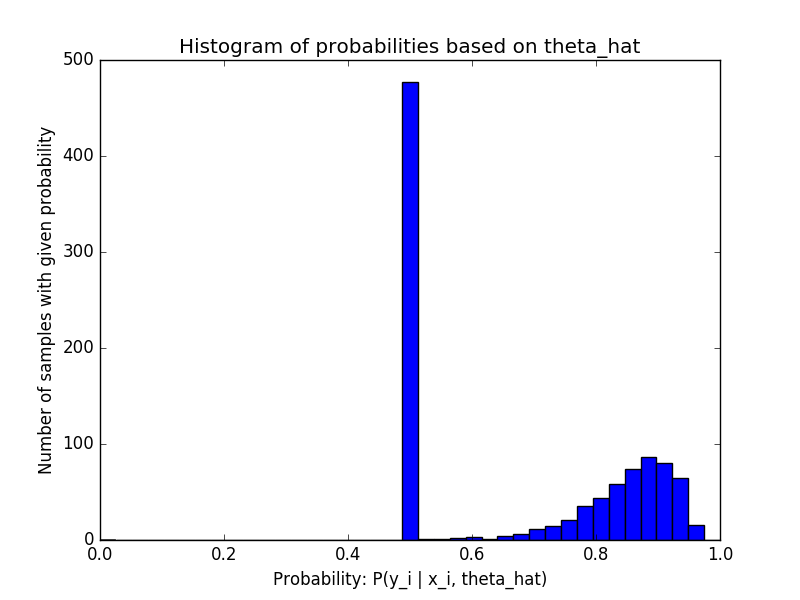
\includegraphics[scale=0.5]{figs/4c.png}
  \caption{Histogram of probabilities using Xone.dat and yone.dat}
  \label{fig:4c}
\end{figure}

(d) Figure \ref{fig:4d} shows a histogram plot of the probabilities $P[y_i | x_i;\hat{\theta}]$  based on fitted vector $\hat{\theta}$ and files Xtwo.dat and ytwo.dat. {\color{red} The differences in Figure \ref{fig:4c} and \ref{fig:4d} are [~~~~~~~~~] and suggest about the accuracy of the fits.}
\begin{figure}[h!]
  \centering
  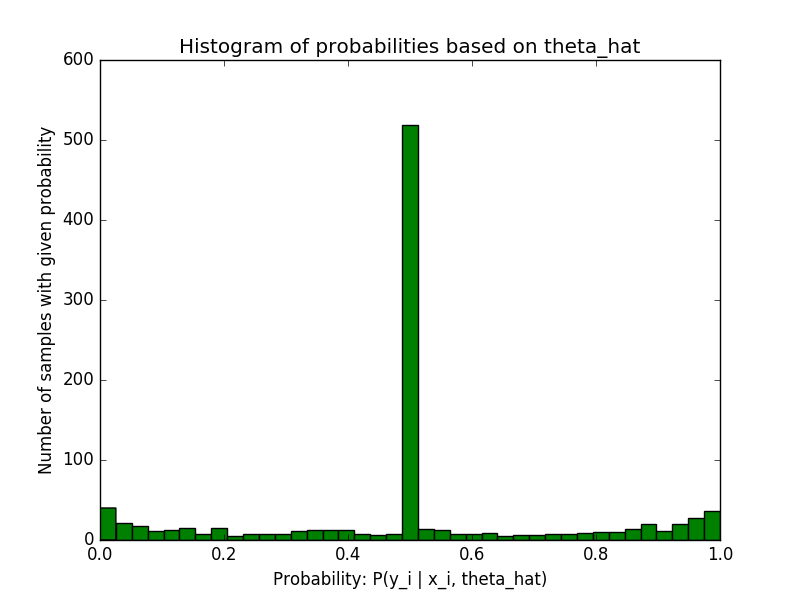
\includegraphics[scale=0.5]{figs/4d.png}
  \caption{Histogram of probabilities using Xtwo.dat and ytwo.dat}
  \label{fig:4d}
\end{figure}

{\color{red}(e) (f)}

\end{problem}

\end{document}